\documentclass[11pt]{article}
\usepackage{graphicx}
\usepackage{fancyhdr}
\usepackage{wrapfig}
\usepackage{hyperref}
\usepackage{tabularx}
\usepackage{setspace}

\newsavebox\CBox
\def\textBF#1{\sbox\CBox{#1}\resizebox{\wd\CBox}{\ht\CBox}{\textbf{#1}}}

\newenvironment{myenv}[1]
  {\begin{spacing}{#1}}
  {\end{spacing}}

\addtolength{\textwidth}{0.2cm}
\setlength{\parskip}{13pt}
\setlength{\parindent}{0.0cm}
\linespread{1.25}

\pagestyle{fancy}
\fancyhf{}
\rhead{TP - Cipullo, Sullivan}
\lhead{Probalidad y Estad\'istica}
\rfoot{\vspace{1cm} \thepage}

\renewcommand*\contentsname{\LARGE Índice}

\begin{document}

\begin{titlepage}
    \begin{center}
        \vfill
        \vfill
            \vspace{0.7cm}
            \noindent\textbf{\Huge Trabajo Pr\'actico}\par
            \noindent\textbf{\Huge Estad\'istica Descriptiva}\par
            \vspace{.5cm}
        \vfill
        \noindent \textbf{\huge Alumnas:}\par
        \vspace{.5cm}
        \noindent \textbf{\Large Cipullo, In\'es}\par
        \noindent \textbf{\Large Sullivan, Katherine}\par
 
        \vfill
        \large Universidad Nacional de Rosario \par
        \noindent\large 2021
    \end{center}
\end{titlepage}
\par

El presente informe tiene como objetivo la exposici\'on de un an\'alisis estad\'istico descriptivo
sobre los datos recopilados del sistema de bicicletas compartidas de la Ciudad de Buenos Aires, EcoBici.

\section{Sobre los datos}
Los datos utilizados se encontraban divididos en dos unidades de an\'alisis diferentes: una correspondiente
a la informaci\'on sobre los usuarios del sistema en el a\~{n}o 2020, y la otra, a la informaci\'on sobre los recorridos 
realizados por los mismos, en el a\~{n}o 2020.
\par
Se cuenta para el siguienete an\'alisis con una muestra aleatoria de 100 usuarios
tomados de las observaciones totales registradas por el Ministerio de Desarrollo Urbano y Transporte de la
Ciudad de Buenos Aires, disponibles en {\small \url{https://data.buenosaires.gob.ar/dataset/estaciones-bicicletas-publicas}}.
\par
Todos los datos y gr\'aficos presentados a continuaci\'on provienen de esta misma y \'unica fuente.

\section{Sobre las variables}
Como fue mencionado en la secci\'on anterior, la informaci\'on se encontraba dividida en dos unidades de an\'alisis.
Cada una de ellas presenta diferentes variables que ser\'an el objeto de inter\'es de este informe.
\par
En la primer unidad (referida a informaci\'on de usuario) se cuenta con tres variables: 
\begin{itemize}
    \item ID de usuario (n\'umero de 6 d\'igitos que identifica un usuario), 
    \item G\'enero de usuario (pudiendo tomar las categor\'ias Femenino, Masculino y Otro), y
    \item Edad de usuario (representada en a\~{n}os).
\end{itemize}

\par
En la segunda unidad (referida a informaci\'on de recorridos) se cuenta con 5 variables: 

\begin{itemize}
    \item Duraci\'on del recorrido(representada en segundos), 
    \item Distancia (distancia entre la estaci\'on de origen y la de destino, representada en metros), 
    \item D\'ia (d\'ia de la semana en el que se realizo el recorrido), 
    \item Direcci\'on de origen (direcci\'on de la estaci\'on de EcoBici desde donde se inici\'o el recorrido), y
    \item Direcci\'on de destino (direcci\'on de la estaci\'on de EcoBici desde donde finaliz\'o el recorrido). 
\end{itemize}

\section{An\'alisis univariado}

\subsection{G\'enero de usuario}

Cabe mencionar antes de proceder al an\'alisis de la variable que la categor\'ia "Otro" es el valor por defecto
al ingresar los datos de usuario, por lo tanto resulta posible que usuarios que se identifiquen con cualquiera
de las otras dos categor\'ias hayan quedado bajo la categor\'ia "Otro" por simplemente no modificar el valor por defecto.

Para comenzar el an\'alisis, se puede observar la siguiente tabla de frecuencias sobre la variable
g\'enero de usuario. 


\begin{center}
\large\textbf{G\'enero de los Usuarios del 
Sistema EcoBici de CABA}

\begin{tabularx} {0.8\textwidth}{ 
    | >{\raggedright\arraybackslash}X 
    | >{\raggedleft\arraybackslash}X 
    | >{\raggedleft\arraybackslash}X | }
   \hline
   \textbf{G\'enero de usuario} & \textbf{Frecuencia absoluta} & \textbf{Frecuencia relativa} \\
   \hline
   Femenino & 38 & 0.38 \\
   \hline
   Masculino & 27 & 0.27 \\
   \hline
   Otro & 35 & 0.35 \\
   \hline \hline
   \textbf{Total} & 100 & 1.00 \\
   \hline
  \end{tabularx}
\end{center}


  Esta informaci\'on, dada la condici\'on cualitativa de la variable, se puede exponer
  en forma de gr\'afico de sectores. As\'i se puede visualizar claramente la porci\'on del
  total que representa cada valor de la variable.
    
  \hspace{-2.3cm}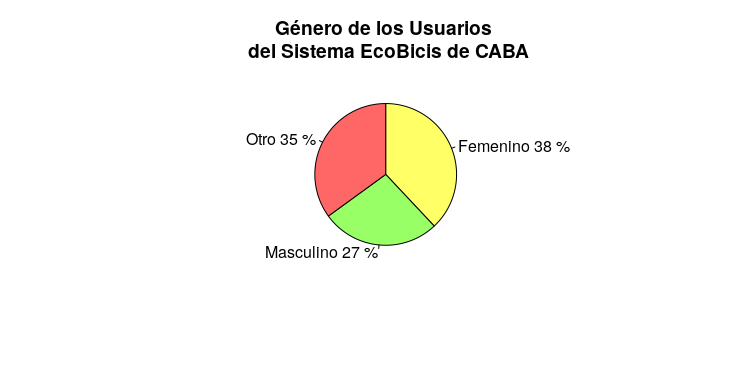
\includegraphics[scale=0.9]{PieChartGenero.png}
  \vspace{-2.5cm}

  De lo descripto se puede observar que las categor\'ias se encuentran bastante uniformemente
  divididas, y que la moda es Femenino, es decir, se cuenta con más usuarios del género Feminino que de cualquiera de los otros.

  \subsection{Edad de usuario}

  Es importante tener en cuenta que para este an\'alisis univariado se cuenta con un total de 99 usuarios,
  puesto que se debi\'o excluir de los datos 
  recopilados un usuario cuyo valor de Edad se presentaba como faltante.

  Se procedi\'o a la divisi\'on de la variable en intervalos de 5 a\~{n}os de edad
  quedando su tabla de frecuencias de la siguiente manera: 

    \begin{center}
        \large\textbf{Edad de los Usuarios del 
        Sistema EcoBici de CABA}
    \end{center}

  \begin{myenv}{1}
    \begin{tabularx} {1\textwidth}{ 
        | >{\raggedright\arraybackslash}X 
        | >{\raggedleft\arraybackslash}X 
        | >{\raggedleft\arraybackslash}X 
        | >{\raggedleft\arraybackslash}X 
        | >{\raggedleft\arraybackslash}X |}
       \hline
       \textbf{Edad de usuario} & \textbf{Frecuencia absoluta} & \textbf{Frecuencia relativa} & \textbf{Frecuencia absoluta acumulada} & \textbf{Frecuencia relativa acumulada} \\
       \hline
       [18,23) & 16 & 0.16 & 16 & 0.16 \\
       \hline
       [23,28) & 15 & 0.15 & 31 & 0.31 \\
       \hline
       [28,33) & 27 & 0.27 & 58 & 0.58 \\
       \hline
       [33,38) & 17 & 0.17 & 75 & 0.75 \\
       \hline
       [38,43) & 12 & 0.12 & 87 & 0.88 \\
       \hline
       [43,48) & 1 & 0.01 & 88 & 0.89 \\
       \hline
       [48,53) & 6 & 0.06 & 94 & 0.95 \\
       \hline
       [53,58) & 3 & 0.03 & 97 & 0.98 \\
       \hline
       [58,63) & 1 & 0.01 & 98 & 0.99 \\
       \hline
       [63,68) & 1 & 0.01 & 99 & 1.00 \\
       \hline \hline
       \textbf{Total} & 99 & 1.00 & - & - \\
       \hline
      \end{tabularx}
    \end{myenv}

    \vspace{5mm}

    Manteniendo esta separaci\'on en intervalos se puede visualizar m\'as c\'omodamente esta informaci\'on en un histograma
    que toma como unidad el intervalo de 5 a\~{n}os, as\'i pudiendo presentar la densidad de las \'areas con
    la cantidad de usuarios.

    \hspace{7mm}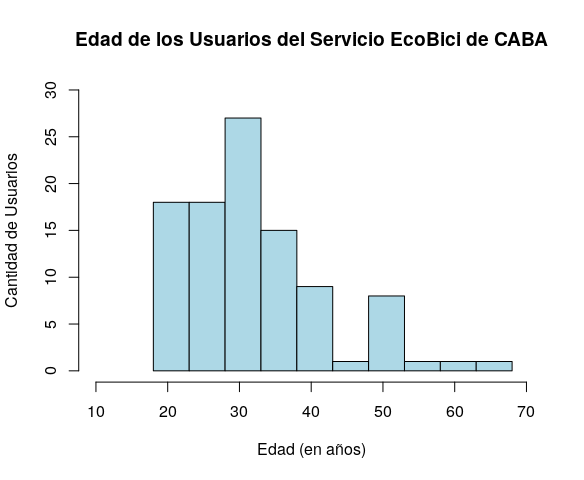
\includegraphics[scale=0.7]{HistEdad.png}

    Acompañando al histograma, tambi\'en resulta \'util la presentaci\'on del pol\'igono de frecuencias (arriba) y el pol\'igono acumulativo (abajo).

    \begin{center}
    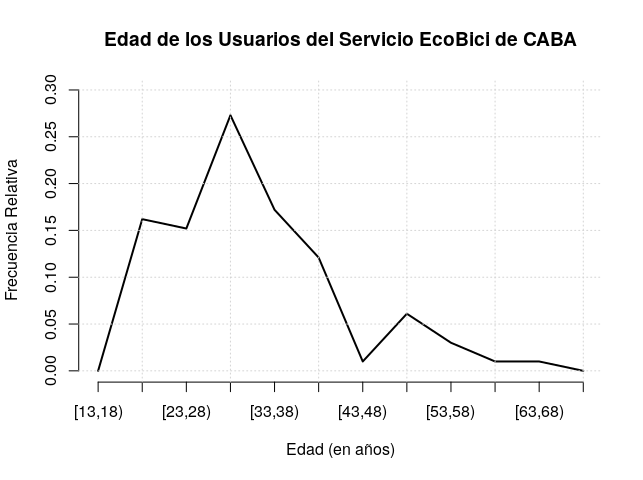
\includegraphics[scale=0.55]{PoligFrecEdad.png}
    \vspace{-4mm}

    (a) Pol\'igono de frecuencias
    \end{center}

    \begin{center}
    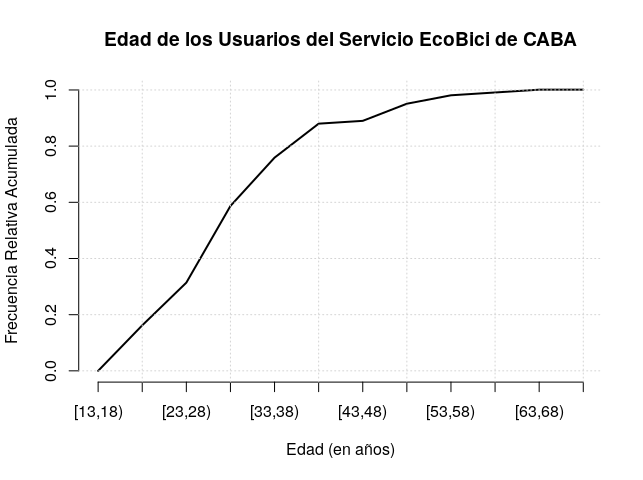
\includegraphics[scale=0.55]{PoligAcumEdad.png}
    \vspace{-4mm}

    (b) Pol\'igono acumulativo
    \end{center}

    Por \'ultimo, dada la condici\'on cuantitativa de la variable edad resulta interesante hablar sobre sus medidas resumen y respectivas medidas de dispersi\'on. 

    La media es de 32.51 a\~{n}os con un desv\'io est\'andar de 9.95 a\~{n}os.

    La mediana la marca la edad de 31 a\~{n}os. El primer cuartil, los 25 a\~{n}os y el tercer cuartil, los 37 a\~{n}os. Por lo tanto se cuenta con un rango intercuartil de 12 a\~{n}os. 

    La edad m\'inima presentada fue de 19 a\~{n}os y la m\'axima, de 66 a\~{n}os.


  \subsection{D\'ia de recorrido}
  Para dar comienzo al an\'alisis univariado de las variables referidas a los recorridos realizados por los 100 usuarios que 
  comprenden la muestra, resulta pertinente mencionar que se cuenta con un total de 411 recorridos. Este ser\'a referido como total para estos an\'alisis. 

  La variable D\'ia de recorrido cuenta con 7 categor\'ias: Domingo, Lunes, Martes, Mi\'ercoles, Jueves, Viernes y S\'abado, y su tabla de frecuencia es la que se presenta a continuaci\'on. 

  \begin{center}
    \large\textbf{Recorridos por d\'ia de semana del Sistema EcoBici de CABA}
    
    \begin{tabularx} {0.8\textwidth}{ 
        | >{\raggedright\arraybackslash}X 
        | >{\raggedleft\arraybackslash}X 
        | >{\raggedleft\arraybackslash}X | }
       \hline
       \textbf{D\'ia} & \textbf{Frecuencia absoluta} & \textbf{Frecuencia relativa} \\
       \hline
       Domingo & 63 & 0.15 \\
       \hline
       Lunes & 63 & 0.15 \\
       \hline
       Martes & 54 & 0.13 \\
       \hline
       Mi\'ercoles & 51 & 0.12 \\
       \hline
       Jueves & 59 & 0.14 \\
       \hline 
       Viernes & 53 & 0.13 \\
       \hline 
       S\'abado & 68 & 0.17 \\
       \hline \hline
       \textbf{Total} & 411 & 1.00 \\
       \hline
      \end{tabularx}
    \end{center}

    Se puede visualizar mejor esta informaci\'on en el gr\'afico de barras que aparece a continuaci\'on. 

    \hspace{7mm}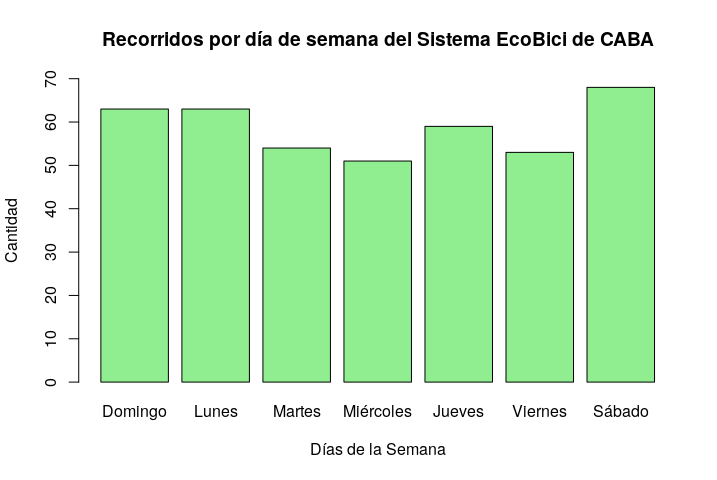
\includegraphics[scale=0.65]{BarPlotDia.png}

    De lo anterior resulta simple notar que la moda de la variable es S\'abado y que la categor\'ia con menor cantidad de recorridos es Mi\'ercoles, aunque, de cualquier manera, las categor\'ias no presentan una gran diferencia entre sus valores.
  
    \subsection{Estaci\'on de origen de recorrido}

    Tomando en consideraci\'on que se cuenta con 142 estaciones se decidi\'o presentar dentro del informe un cuadro con las 10 estaciones que fueron utilizadas m\'as veces como origen por la muestra de usuarios. 
    Si se desea obtener el cuadro de frecuencias completo puede acceder a \'el mediante el siguiente enlace {\small \url{https://data.buenosaires.gob.ar/dataset/estaciones-bicicletas-publicas}}

    Entonces, por un lado, recordando que no se llegan al total esperado de 411 recorridos porque solo presentamos las 10 con mayor frecuencia, se presenta la tabla a continuaci\'on. 




    Visualizando esta tabla resulta claro que la moda es la estaci\'on ubicada en Ramos Mejia, Av Dr Jose Maria Vargas \& Av. Del Libertador. 

    Sin embargo, por otro lado, teniendo en cuenta la cantidad de estaciones se vio como pertinente el recategorizar la variable 
    con respecto a la cantidad de estaciones utilizadas como origen una x cantidad de veces. Es decir, 
    las categor\'ias nuevas tendr\'an la forma de un n\'umero x que representa la cantidad de recorridos iniciados y su valor
    asociado ser\'a la cantidad de estaciones que hayan sido origen de esa x cantidad de recorridos. 

    Una vez hecha esta recategorizaci\'on se hace f\'acil de reconocer el principio de Paretto que aparece: las categor\'ias con n\'umeros m\'as bajos son las que 
    agrupan la mayor cantidad de estaciones, lo cual se puede observar claramente en el siguiente gr\'afico de Paretto. 




    \subsection{Estaci\'on de destino de recorrido}

    Tomando en consideraci\'on que se cuenta con 135 estaciones se decidi\'o presentar dentro del informe un cuadro con las 10 estaciones que fueron utilizadas m\'as veces como destino por la muestra de usuarios. 
    Si se desea obtener el cuadro de frecuencias completo puede acceder a \'el mediante el siguiente enlace {\small \url{https://data.buenosaires.gob.ar/dataset/estaciones-bicicletas-publicas}}

    Entonces, por un lado, recordando que no se llegan al total esperado de 411 recorridos porque solo presentamos las 10 con mayor frecuencia, se presenta la tabla a continuaci\'on. 




    Visualizando esta tabla resulta claro que la moda es la estaci\'on ubicada en Lavalle \& Bouchard. 

    Sin embargo, por otro lado, teniendo en cuenta la cantidad de estaciones y lo realizado con la variable anterior se vio como pertinente el recategorizar la variable 
    con respecto a la cantidad de estaciones utilizadas como origen una x cantidad de veces. Es decir, 
    las categor\'ias nuevas tendr\'an la forma de un n\'umero x que representa la cantidad de recorridos iniciados y su valor
    asociado ser\'a la cantidad de estaciones que hayan sido origen de esa x cantidad de recorridos. 

    Otra vez, ya hecha esta recategorizaci\'on se hace f\'acil de reconocer el principio de Paretto que aparece: las categor\'ias con n\'umeros m\'as bajos son las que 
    agrupan la mayor cantidad de estaciones, lo cual se puede observar en el siguiente gr\'afico de Paretto. 


\end{document}                                                                                  